\documentclass[12pt,letterpaper]{exam}
\usepackage[lmargin=1in,rmargin=1in,tmargin=1in,bmargin=1in]{geometry}
\usepackage{../style/exams}

% -------------------
% Course & Exam Information
% -------------------
\newcommand{\course}{MATH 111I: Final Exam}
\newcommand{\term}{Spring --- 2025}
\newcommand{\examdate}{05/01/2025}
\newcommand{\timelimit}{150 Minutes}

\setbool{hideans}{false} % Student: True; Instructor: False

% -------------------
% Content
% -------------------
\begin{document}

\examtitle
\instructions{Write your name on the appropriate line on the exam cover sheet. This exam contains \numpages\ pages (including this cover page) and \numquestions\ questions. Check that you have every page of the exam. Answer the questions in the spaces provided on the question sheets. Be sure to answer every part of each question and show all your work. If you run out of room for an answer, continue on the back of the page --- being sure to indicate the problem number.} 
\scores
\bottomline
\newpage


% -------------------
% Questions
% -------------------
\begin{questions}

% Question 1
\newpage
\question[6] Find the average rate of change of $f(x)= 2x^2 - 4x + 5$ on the interval $[-1, 2]$. \pspace

\ans{\newline Recall that the average rate of change of a function $f(x)$ on an interval $[a, b]$ is $\dfrac{f(b) - f(a)}{b - a}$. We have $a= -1$, $b= 2$, and $f(x)= 2x^2 - 4x + 5$. But then\dots \pspace
	\[
	\begin{aligned}
	f(-1)&= 2(-1)^2 - 4(-1) + 5= 2(1) - (-4) + 5= 2 + 4 + 5= 11 \\[0.5cm]
	f(2)&= 2(2^2) - 4(2) + 5= 2(4) - 4(2) + 5= 8 - 8 + 5= 5
	\end{aligned}
	\] \pspace
Therefore, the average rate of change of $f(x)= 2x^2 - 4x + 5$ on the interval $[-1, 2]$ is\dots
	\[
	\text{Avg. ROC}= \dfrac{f(2) - f(-1)}{2 - (-1)}= \dfrac{11 - 5}{2 + 1}= \dfrac{6}{3}= 2
	\]
}



% Question 2
\newpage
\question[6] Consider the graph of the relation $f(x)$ below. 
	\[
	\fbox{
	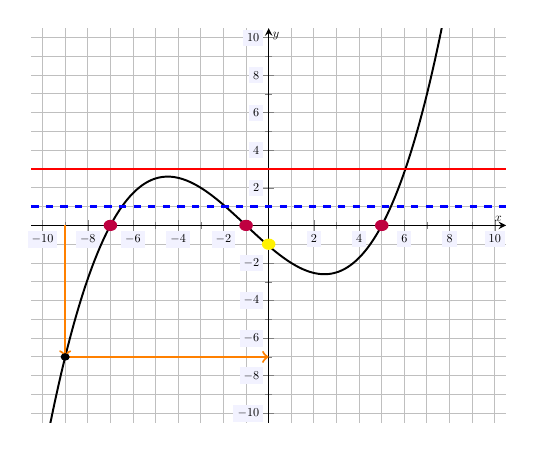
\begin{tikzpicture}[scale=0.88,every node/.style={scale=0.5}]
	\begin{axis}[
	grid=both,
	axis lines=middle,
	ticklabel style= {fill= blue!5!white},
	xmin= -10.5, xmax=10.5,
	ymin= -10.5, ymax=10.5,
	xtick= {-10,-8,...,10},
	ytick= {-10,-8,...,10},
	minor tick = {-10,-9,...,10},
	xlabel= \(x\), ylabel= \(y\)
	]
	\addplot[thick, samples=100, smooth, domain= -10.5:10.5] {1/32*(x^3 + 3*x^2 - 33*x - 35)};
	\remove{\draw[line width=0.04cm,blue,dashed] (-10.5,1) -- (10.5,1);}
	\remove{\draw[draw=none,fill=purple] (-7,0) circle (0.3);}
	\remove{\draw[draw=none,fill=purple] (-1,0) circle (0.3);}
	\remove{\draw[draw=none,fill=purple] (5,0) circle (0.3);}
	\remove{\draw[draw=none,fill=yellow] (0,-1) circle (0.3);}
	\remove{\draw[line width=0.03cm,orange,->] (-9,0) -- (-9,-7);}
	\remove{\draw[line width=0.03cm,orange,->] (-9,-7) -- (0,-7);}
	\remove{\draw[draw=none,fill=black] (-9,-7) circle (0.2);}
	\remove{\draw[line width=0.04cm,red] (-10.5,3) -- (10.5,3);}
	\end{axis}
	\end{tikzpicture}
	}
	\]

\begin{enumerate}[(a)]
\item Is $f(x)$ a function? Explain why or why not. \pspace
\ans{Yes, $f(x)$ is a function because it passes the vertical line test, i.e. every vertical line intersects the graph of $f(x)$ at most once.} \pspace

\item Does $f(x)$ have an inverse? Explain why or why not. \pspace
\ans{No, $f(x)$ does not have an inverse because it fails the horizontal line test, i.e. not every horizontal line intersects the function at most once. For instance, the horizontal line at $y= 1$ (the blue line) intersects $f(x)$ more than once.} \pspace

\item Find the root(s) for $f(x)$. \pspace
\ans{The root(s) for $f(x)$ are $x$-values such that $f(x)= 0$, i.e. where the graph of $f(x)$ crosses the $x$-axis. From the plot, we can see that this is at $x= -7, -1, 5$.} \pspace

\item Find the $y$-intercept for $f(x)$. \pspace
\ans{This is the $y$-value---or point---where the plot of $f(x)$ intersects the $y$-axis. From the plot, we can see this is at $y= -1$. Alternatively, the $y$-intercept is $(0, -1)$.} \pspace

\item Find $f(-9)$. \pspace
\ans{This is the $y$-value when $x= -2$. From the plot, we can see that $f(-9)= -7$.} \pspace

\item Solve the equation $f(x)= 3$. \pspace
\ans{The solutions to $f(x)= 3$ are $x$-values where the output is 3. These will be points such that the $y$-value is 7. Drawing the line $y= 3$---the red line---we can see that this intersects the graph of $f(x)$ at $x= 3$. From the plot, we can see that this is at $x= 6$.}
\end{enumerate}



% Question 3
\newpage
\question[6] Find the equation of the line through the $y$-intercept of $y= 3x - 5$ that is parallel to the line $y= 9 - 6x$. \pspace

\ans{The $y$-intercept of the line $y= 3x - 5$ is $(0, -5)$. Therefore, the desired line contains the point $(0, -5)$. We know that parallel lines have equal slopes. The slope of the line $y= 9 - 6x$ is $-6$. Therefore, the slope of the desired line is $-6$. But then the desired line contains $(x_0, y_0)= (0, -5)$ and has slope $m= -6$. Using point-slope form, we have\dots \pspace
	\[
	\begin{gathered}
	y= y_0 + m(x - x_0) \\[0.5cm]
	y= -5 + -6(x - 0) \\[0.5cm]
	y= -5 - 6x
	\end{gathered}
	\]
}



% Question 4
\newpage
\question[6] A band receives a flat performance payment of \$15,000. They also receive 15\% of each of the \$60 tickets sold. Let $M(T)$ be the amount of money the band makes in total for their performance if $T$~tickets are sold. 
	\begin{enumerate}[(a)]
	\item Explain why $M(T)$ is linear. \pspace
	\ans{We know that a function is linear if and only if they have a constant rate of change. The only way the band makes more money is by selling more tickets. But they receive the same amount per ticket sold. Therefore, the rate of change in the amount the band makes is constant. Therefore, the amount of money the band makes, $M(T)$, is a linear function.} \pvspace{3cm}
	
	\item Find $M(T)$. \pspace
	\ans{We know from (a) that $M(T)$ is linear. Therefore, $M(T)= mT + b$ for some $m, b$. The band makes 15\% of each of the \$60 tickets sold. We know that 15\% of \$60 is $60(0.15)= 9$. This is the rate of change of $M(T)$. Therefore, $m= 9$. This shows that $M(T)= mT + b= 9T + b$. We know that the band makes \$15,000 even if no tickets are sold, i.e. $M(0)= 15000$. But then $15000= M(0)= 9(0) + b= 0 + b= b$. This shows that $b= 15000$. Therefore, we have\dots
		\[
		M(T)= 9T + 15000
		\]
	}
	\end{enumerate}



% Question 5
\newpage
\question[6] The population of a town $y$~years from now, $P(y)$, is a linear function of time. The Census Bureau determines that $P(y)= 35000 - 670y$. 
	\begin{enumerate}[(a)]
	\item Find and interpret the $y$-intercept of $P(y)$. \pspace
	\ans{Given a linear function of the form $y= mx + b$, the $y$-intercept is $b$. We have $P(y)= 35000 - 670y= -670y + 35000$. This shows that $b= 35000$. \pspace
	
	The $y$-intercept is the output when the input is $0$. But then $P= 35000$ when $y= 0$. So, $y= 0$~years from now, the population will be $P= 35000$; that is, the current population of the town is 35,000 individuals.} \vfill

	\item Find an interpret the slope of $P(y)$. \pspace
		\ans{Given a linear function of the form $y= mx + b$, the slope is $m$. We have $P(y)= 35000 - 670y= -670y + 35000$. This shows that $m= -670$. \pspace
	
	Because $m= -670 < 0$, we know that $P(y)$ is decreasing. We know that $m= \dfrac{\Delta P}{\Delta y}= -670= \dfrac{-670}{1}$. Therefore, each increase of 1 in $y$ results in a decrease of 670 in $P$; that is, every year the population of the town decreases by 670~individuals.} \vfill
	
	\item When will the town have 25,000~people in it? \pspace
	\ans{We want a year $y$ when $P(y)= 25000$. But then\dots
		\[
		\begin{gathered}
		P(y)= 25000 \\[0.4cm]
		35000 - 670y= 25000 \\[0.4cm]
		-670y= -10000 \\[0.4cm]
		y \approx 14.93
		\end{gathered}
		\]
	Therefore, the population of the town will be 25,000 approximately 14.93~years from now.} \vfill
	\end{enumerate}



% Question 6
\newpage
\question[6] Showing all your work, factor the following as completely as possible:
	\begin{enumerate}[(a)]
	\item $x^2 - 9$ \pspace
	\ans{Recall difference of perfect squares: $a^2 - b^2= (a - b)(a + b)$. We have $a= x$ and $b= 3$, i.e. $a^2= x^2$ and $b^2= 9$. But then\dots
		\[
		x^2 - 9= (x - 3)(x + 3)
		\]
	}

	\item $x^2 - 2x - 24$ \pspace
	\ans{We find factors of $-24$ that add to $-2$. Because $-24 < 0$, the factors must have opposite signs.
	\begin{table}[!ht]
	\centering
	\wsol{\underline{\bfseries $\mathbf{-24}$}} \pvspace{0.2cm}
	\begin{tabular}{rrrrr}
	\wsol{$1 \cdot -24$} & \wsol{$-23$} & \hspace{0.4cm} & \wsol{$3 \cdot -8$} & \wsol{$-5$} \\
	\wsol{$-1 \cdot 24$} & \wsol{$23$} & & \wsol{$-3 \cdot 8$} & \wsol{$5$} \\
	\wsol{$2 \cdot -12$} & \wsol{$-10$} & & \wsol{\underline{$\mathbf{4 \cdot -6}$}} & \wsol{\underline{$\mathbf{-2}$}} \\
	\wsol{$-2 \cdot 12$} & \wsol{$10$} & & \wsol{$-4 \cdot 6$} & \wsol{$2$} 
	\end{tabular}
	\end{table} \par
	Therefore, we have\dots
		\[
		x^2 - 2x - 24= \boxed{(x + 4)(x - 6)}
		\] 
	}
	
	\item $6x^2 + 19x + 10$ \pspace
	\ans{We find factors of $6 \cdot 10= 60$ that add to $19$. Because $10 > 0$, the factors must have the same sign.
	\begin{table}[!ht]
	\centering
	\wsol{\underline{\bfseries $\mathbf{60}$}} \pvspace{0.2cm}
	\begin{tabular}{rrrrr}
	\wsol{$1 \cdot 60$} & \wsol{$61$} & \hspace{0.4cm} & \wsol{\underline{$\mathbf{4 \cdot 15}$}} & \wsol{\underline{$\mathbf{19}$}} \\
	\wsol{$-1 \cdot -60$} & \wsol{$-61$} & & \wsol{$-4 \cdot -15$} & \wsol{$-19$} \\
	\wsol{$2 \cdot 30$} & \wsol{$32$} & & \wsol{$5 \cdot 12$} & \wsol{$17$} \\
	\wsol{$-2 \cdot -30$} & \wsol{$-32$} & & \wsol{$-5 \cdot -12$} & \wsol{$-17$} \\
	\wsol{$3 \cdot 20$} & \wsol{$23$} & & \wsol{$6 \cdot 10$} & \wsol{$16$} \\
	\wsol{$-3 \cdot -20$} & \wsol{$-23$} & & \wsol{$-6 \cdot -10$} & \wsol{$-16$} 
	\end{tabular}
	\end{table} \par
	Therefore, we have\dots
		\[
		6x^2 + 19x + 10= 6x^2 + 4x + 15x + 10= 2x(3x + 2) + 5(3x + 2)= (3x + 2)(2x + 5)
		\] \vfill
	}
	\end{enumerate} 



% Question 7
\newpage
\question[6] Showing all your work, solve the following quadratic equation using the quadratic formula:
	\[
	1= x(4 - x)
	\] \pspace

\ans{We have\dots
	\[
	\begin{gathered}
	1= x(4 - x) \\[0.3cm]
	1= 4x - x^2 \\[0.3cm]
	x^2 - 4x + 1= 0 
	\end{gathered}
	\] \pspace
The function $x^2 - 4x + 1$ is quadratic function with $a= 1$, $b= -4$, and $c= 1$. Using the quadratic formula, we have\dots \pspace
	\[
	\begin{aligned}
	x&= \dfrac{-b \pm \sqrt{b^2 - 4ac}}{2a} \\[0.3cm]
	&= \dfrac{-(-4) \pm \sqrt{(-4)^2 - 4(1)1}}{2(1)} \\[0.3cm]
	&= \dfrac{4 \pm \sqrt{16 - 4}}{2} \\[0.3cm]
	&= \dfrac{4 \pm \sqrt{12}}{2} \\[0.3cm]
	&= \dfrac{4 \pm \sqrt{4 \cdot 3}}{2} \\[0.3cm] 
	&= \dfrac{4 \pm 2 \sqrt{3}}{2} \\[0.3cm]  
	&= 2 \pm \sqrt{3}
	\end{aligned}
	\]
}



% Question 8
\newpage
\question[6] Find the domain of the following functions:
	\begin{enumerate}[(a)]
	\item $f(x)= x^3 - 4x + 9$ \pspace
	\ans{We know $f(x)$ is a polynomial. The domain of any polynomial is all real numbers, i.e. $\mathbb{R}$ or $(-\infty, \infty)$.} \vfill
	
	\item $g(x)= \sqrt{x + 8}$ \pspace
	\ans{For an even root to be defined, the `inside' needs to be nonnegative. But then $x + 8 \geq 0$, which implies $x \geq -8$. Therefore, the domain of $g(x)$ is $[-8, \infty)$.} \vfill
	
	\item $h(x)= \dfrac{x + 5}{x + 4}$ \pspace
	\ans{For a `fraction' to be defined, the denominator cannot be 0. If $x + 4= 0$, then $x= -4$. Therefore, the domain of $h(x)$ is the set of real numbers not equal to $-4$, i.e. $\mathbb{R} \setminus \{ -4 \}$ or $(-\infty, -4) \cup (-4, \infty)$.} \vfill
	
	\item $j(x)= \ln(x - 6)$ \pspace
	\ans{For a logarithm to be defined, the `inside' needs to be positive. But then $x - 6 > 0$, which implies $x > 6$. Therefore, the domain is $(6, \infty)$.} \vfill
	
	\item $k(x)= 6e^{3x}$ \pspace
	\ans{The domain of any exponential function $y= Ab^x$ is the set of all real numbers. Therefore, the domain of $k(x)$ is the set of all real numbers, i.e. $\mathbb{R}$ or $(-\infty, \infty)$.} \vfill
	\end{enumerate}



% Question 9
\newpage
\question[6] Find functions $f(x)$ and $g(x)$ so that the following functions can be written in the form $f \big( g(x) \big)$: \pvspace{0.2cm}
	\begin{enumerate}[(a)]
	\item $e^{x - x^2}$ \pspace
	\ans{There are infinitely many solutions. For instance, we can choose\dots
		\[
		\boxed{%
		\begin{aligned}
		f(x)&= e^x \\[0.2cm]
		g(x)&= x - x^2
		\end{aligned}}
		\] \vfill
	}

	\item $7(2x + 3)^9$ \pspace
	\ans{There are infinitely many solutions. For instance, we can choose\dots
		\[
		\boxed{%
		\begin{aligned}
		f(x)&= 7x^9 \\[0.2cm]
		g(x)&= 2x + 3
		\end{aligned}}
		\] \vfill
	}

	\item $\dfrac{1}{\ln(x)}$ \pspace
	\ans{There are infinitely many solutions. For instance, we can choose\dots
		\[
		\boxed{%
		\begin{aligned}
		f(x)&= \dfrac{1}{x} \\[0.2cm]
		g(x)&= \ln x
		\end{aligned}}
		\] \vfill
	}
	\end{enumerate}



% Question 10
\newpage
\question[6] Showing all your work, find the vertex for $x^2 + 8x + 13$. \pspace

\ans{By completing the square, we first take half the `middle term', $\frac{8}{2}= 4$, square this value, $4^2= 16$, and add/subtract this value. This yields\dots
	\[
	x^2 + 8x + 13= x^2 + 8x + 16 - 16 + 13= (x^2 + 8x + 16) + (-16 + 13)= (x + 4)^2 - 3
	\] \pspace
Therefore, the vertex is $(-4, -3)$ and because $a= 1 > 0$, the parabola opens upwards. \pspace

Using the `evaluation method', we know the $x$-coordinate of the vertex is $x= -\frac{b}{2a}$. This is a quadratic function with $a= 1$, $b= 8$, and $c= 13$. But then the $x$-coordinate of the vertex is $x= -\frac{8}{2(1)}= -\frac{8}{2}= -4$. But then the $y$-coordinate of the vertex is\dots
	\[
	x^2 + 8x + 13 \bigg|_{x= -4}= (-4)^2 + 8(-4) + 13= 16 - 32 + 13= -3
	\]
This shows that the vertex is $(-4, -3)$. We know the vertex form of a quadratic function is $a(x - P)^2 + Q$, where $a$ is from the standard form and $(P, Q)$ is the vertex. We have $a= 1$ and $(P, Q)= (-4, -3)$. Therefore, we have\dots
	\[
	a(x - P)^2 + Q= 1 \big(x - (-4) \big)^2 + (-3)= (x + 4)^2 - 3
	\]
}



% Question 11
\newpage
\question[6] Consider the exponential function $y= 6(3^{2x - 1})$.
	\begin{enumerate}[(a)]
	\item Write this exponential function in the form $y= Ab^x$. \pspace
	\ans{We have\dots
		\[
		y= 6(3^{2x - 1})= 6(3^{2x} \cdot 3^{-1})= 6 (3^2)^x \cdot \dfrac{1}{3^1}= \dfrac{6}{3} (9^x)= 2(9^x)
		\]
	We have $y= 2(9^x)$. So, we know here that $A= 2$ and $b= 9$.} \vfill
	
	\item Is $y$ growing or shrinking exponentially? Explain. \pspace
	\ans{For an exponential function $Ab^x$ with $A > 0$, we know that the function is exponentially increasing if $b > 1$ and exponentially decreasing if $0 < b < 1$. From (a), we know that $A= 2 > 0$ and $b= 9 > 1$. Therefore, this function is exponentially increasing.} \vfill
	
	\item Determine the $y$-intercept for this function. \pspace
	\ans{For an exponential function $Ab^x$, the $y$-intercept is $A$. From (a), we know that $A= 2$. Therefore, the $y$-intercept is 2. \pspace
	
	Alternatively, we know the $y$-intercept is the value when the input is 0. We have $y= 6(3^{2(0) - 1})= 6(3^{0 - 1})= 6 (3^{-1})= 6 \cdot \frac{1}{3}= 2$.} \vfill
	\end{enumerate}



% Question 12
\newpage
\question[6] Consider the exponential function $f(x)= 441.3(0.85)^x$.
	\begin{enumerate}[(a)]
	\item What is the `initial value' for $f(x)$? \pspace
	\ans{For an exponential function $Ab^x$ with $A > 0$, we know that the `initial value' is $A$. We know here that $A= 441.3$ and $b= 0.85$. Therefore, the `initial value' is $441.3$. \pspace
	
	Alternatively, we know the `initial value' should be the output when the input is $0$, i.e. $x= 0$. But then the initial value must be $441.3(0.85)^0= 441.3(1)= 441.3$.} \vfill
	
	\item Does $f(x)$ have growing exponentially or decaying exponentially? Explain. \pspace
	\ans{For an exponential function $Ab^x$ with $A > 0$, we know that the function is exponentially increasing if $b > 1$ and exponentially decreasing if $0 < b < 1$. From (a), we know that $A= 441.3 > 0$ and $b= 0.85$ and $0 < b < 1$. Therefore, this function is decaying exponentially.} \vfill
	
	\item Find the growth or decay rate for $f(x)$. \pspace
	\ans{For an exponential function $Ab^x$, if we write $b= 1 \pm g$, where $g > 0$, then the function has growth rate $g$ if we use `$+$' and the function has decay rate $g$ if we use `$-$'. From (a), we know that $A= 441.3$ and $b= 0.85$. We write $b= 1 - 0.15= 0.85$. Because we require `$-$', we know $f(x)$ is decaying---which we found in (b). As $g= 0.15$, we know that the decay rate for $f(x)$ is 15\%.} \vfill
	\end{enumerate}



% Question 13
\newpage
\question[6] Showing all your work, complete the following:
	\begin{enumerate}[(a)]
	\item Rewrite $\log_6(x)= w$ as an exponential equation. \pspace
	\ans{We know that $\log_b(y)= x$ if and only if $b^x= y$. Therefore, $\log_6(x)= w$ written as an exponential equation is\dots
		\[
		6^w= x
		\]
	}
	
	\item Rewrite $e^{4x}= t$ as a logarithmic equation. \pspace
	\ans{We know that $b^x= y$ if and only if $\log_b(y)= x$. Therefore, using the fact that $\log_e x= \ln x$, we know that $e^{4x}= t$ written as a logarithmic equation is\dots
		\[
		\ln(t)= 4x
		\]
	}
	
	\item Compute $\log_4(5)$. \pspace
	\ans{Using the change of base $\log_b x= \frac{\ln x}{\ln b}$, we have\dots
		\[
		\log_4(5)= \dfrac{\ln(5)}{\ln(4)}= \dfrac{1.60944}{1.38629}= 1.16097
		\]
	}
	\end{enumerate}



% Question 14
\question[6] Rewrite each of the following in the form $x^{a/b}$ for some $a, b$.
	\begin{enumerate}[(a)]
	\item $\sqrt[3]{x^7}$ \pspace
	\ans{
		\[
		\sqrt[3]{x^7}= x^{7/3}
		\]
	}
	
	\item $\dfrac{1}{\sqrt{x}}$ \pspace
	\ans{
		\[
		\dfrac{1}{\sqrt{x}}= \dfrac{1}{x^{1/2}}= x^{-1/2}
		\]
	}
	
	\item $\sqrt{x^5}$ \pspace
	\ans{
		\[
		\sqrt{x^5}= x^{5/2}
		\]
	}
	\end{enumerate}



% Question 15
\newpage
\question[6] You invest \$7,000 at 1.2\% annual interest, compounded continuously. 
	\begin{enumerate}[(a)]
	\item How long until the investment is worth \$9,000? \pspace
	\ans{If one invests an initial amount, $P$, i.e. a principal, at an annual interest rate $r$ (expressed as a decimal), compounded continuously, for a total of $t$ years, then the value of the investment is $Pe^{rt}$. The initial investment is $P= 7000$ and the interest rate is $r= 0.012$. If the investment is worth \$9,000, then $Pe^{rt}= 9000$. But then\dots
		\[
		\begin{gathered}
		Pe^{rt}= 9000 \\[0.2cm]
		7000e^{0.012t}= 9000 \\[0.2cm]
		e^{0.012t}= 1.2857143 \\[0.2cm]
		\ln(e^{0.012t})= \ln(1.2857143) \\[0.2cm] 
		0.012t= 0.2513144 \\[0.2cm]
		t \approx 20.94
		\end{gathered}
		\]
	Therefore, the investment will be worth \$9,000 after approximately 20.94~years.} \vfill
	
	\item How much money is the investment worth after 5~years? \pspace
	\ans{We know from (a) that the amount the investment is worth after $t$ years is $Pe^{rt}$, and we know that $P= 7000$ and $r= 0.012$. But then after $t= 5$~years, the investment is worth\dots
		\[
		Pe^{rt}= 7000e^{0.012(5)}= 7000e^{0.06}= 7000(1.0618365465) \approx 7432.86
		\] \pspace
	Therefore, after 5~years, the investment is worth approximately \$7,432.86} \vfill
	\end{enumerate}

\end{questions}
\end{document}